\documentclass[
	%final % Megadásával a teendők elrejtésre kerülnek
]{elteikthesis}[2019/04/30]

% Dolgozat metaadatai
\title{Téradatok verziókövetésének megvalósítása Quantum GIS-ben}
\date{2019}

% Szerző metaadatai
\author{Dorogi Benjámin}
\degree{programtervező informatikus BSc}

% Témavezető(k) metaadatai
\supervisor{Cserép Máté}
\affiliation{egyetemi tanársegéd}
%\extsupervisor{Külső Kornél}
%\extaffiliation{informatikai igazgató}

% Egyetem metaadatai
\university{Eötvös Loránd Tudományegyetem}
\faculty{Informatikai Kar}
\department{Programozáselmélet és Szoftvertechnológiai}
\departmentSecondLine{Tanszék}
\city{Budapest}
\logo{elte_cimer_szines}

% Irodalomjegyzék hozzáadása
\addbibresource{thesis.bib}

% A dolgozat
\begin{document}
	
% Nyelv kiválasztása
\documentlang{magyar}
%\documentlang{english}

% Teendők listája - final dokumentumban nincs	
\listoftodos[\todolabel]

% Lábjegyzet folytonos számozása fejezetek között
\counterwithout{footnote}{chapter}

% Címlap - kötelező
\maketitle

% Tartalomjegyzék - kötelező
\tableofcontents
\cleardoublepage

% Tartalom
\chapter{Bevezetés}
\label{ch:intro}

Az informatikai projekteknek a munkafolyamatok követése, a különböző állapotok megtekintésének és visszaállításának lehetősége kulcsfontosságú részét képezi az agilis projektmenedzsment, valamint a kooperatív és elosztott munkavégzés elősegítése érdekében. Napjainkban a szöveges alapú munkák -- például szoftverkód, szöveges dokumentumok, táblázatok -- esetében már számtalan eszköz áll rendelkezésünkre ezen funkcionalitás eléréséhez. Attól függően, hogy milyen módon tárolják a kezelt állományokat, a verziókezelő rendszereket két részre oszthatjuk. A centralizált verziókezelők egy központi tárhelyen tárolják a fájlokat, és minden felhasználó ezt a központi verziót módosíthatja, ilyen elven működik például az SVN \cite{svn}. Az elosztott revíziókezelők esetében minden felhasználó rendelkezik a követett projekt teljes másolatával, és szerkesztéskor ez módosul, különválasztva a verziókezelési és a hálózati műveleteket. Ilyen rendszerre a legismertebb példa a Git \cite{git}.
Az említett verziókezelők közös tulajdonsága, hogy mind úgynevezett állapot alapú revíziókezelést valósítanak meg, azaz minden egyes módosításkor az állományok nyers változásait, sorok törlését, hozzáadását tárolják, és ezek alapján állítanak elő újabb vagy régebbi revíziókat.

Az állapot alapú verziókezelés egyik hiányossága, hogy az adatokat binárisan tároló folyamatok esetében -- például jellemzően grafikus állományok tárolása esetén --, nagy tárigényű és jóval kevésbé hatékony. Ezen kívül problémát jelent az is, hogy az állapot alapú verziókezelés esetén a módosítások szemantikai információja elvész, nem követhető, hogy pontosan milyen transzformációk kerültek végrehajtásra, függetlenül az adatformátumtól.
Az ilyen téradatok esetében a művelet alapú revíziókezelés sokkal célravezetőbb, mivel ebben az esetben a változások (vagy más szóval \emph{delták}) az adott objektumokon végzett műveletek, melyek újbóli végrehajtásával megkaphatjuk a frissített változatát a módosított adatnak, az invertált műveletek alkalmazásával pedig korábbi állapotokat érhetünk el.
A téradatok hatékony verziókezelésére való igényre válaszként született az Eötvös Loránd Tudományegyetemen fejlesztett \emph{AEGIS} geoinformatikai programcsomag \cite{giachetta2013aegis, aegis} revíziókezelő modulja \cite{cserep2013versioning,cserep2015operation}, ami interfészt biztosít az összes szükséges folyamathoz, viszont ezen szoftvernek még nem született valós, ipari környezetben is felhasználható implementációja.

Szakdolgozatom motivációja az előbbi hiány megszüntetése, a széleskörűen elterjedt és használt nyílt forráskódú \emph{QGIS} térinformatikai programhoz \cite{qgis} írt verziókezelő beépülő modul megvalósításával, mely a \emph{Q-Aegis} nevet kapta.

A modul feladata a \emph{QGIS} alapvető geometriai műveleteinek naplózása, tetszőleges verzióállapotok betöltése az \emph{AEGIS} könyvtár funkcióinak felhasználásával


\cleardoublepage

\chapter{Felhasználói dokumentáció}
\label{ch:user}

Lorem ipsum dolor sit amet, consectetur adipiscing elit. Duis nibh leo, dapibus in elementum nec, aliquet id sem. Suspendisse potenti. Nullam sit amet consectetur nibh. Donec scelerisque varius turpis at tincidunt. Cras a diam in mauris viverra vehicula. Vivamus mi odio, fermentum vel arcu efficitur, lacinia viverra nibh. Aliquam aliquam ante mi, vel pretium arcu dapibus eu. Nulla finibus ante vel arcu tincidunt, ut consectetur ligula finibus. Mauris mollis lectus sed ipsum bibendum, ac ultrices erat dictum. Suspendisse faucibus euismod lacinia. Etiam vel odio ante. Etiam pulvinar nibh quis massa auctor congue. Pellentesque quis odio vitae sapien molestie vestibulum sit amet et quam. Pellentesque vel dui eget enim hendrerit finibus at sit amet libero. Quisque sollicitudin ultrices enim, nec porta magna imperdiet vitae. Cras condimentum nunc dui, eget molestie nunc accumsan vel.

Donec dapibus sodales ante, at scelerisque nunc laoreet sit amet. Mauris porttitor tincidunt neque, vel ullamcorper neque pulvinar et. Integer eu lorem euismod, faucibus lectus sed, accumsan felis. Nunc ornare mi at augue vulputate, eu venenatis magna mollis. Nunc sed posuere dui, et varius nulla. Sed mollis nibh augue, eget scelerisque eros ornare nec. Praesent porta, metus eget eleifend consequat, eros ligula eleifend ex, a pellentesque mi est vitae urna. Vivamus turpis nunc, iaculis non leo eget, mattis vulputate tellus. Maecenas rutrum eros sem, pharetra interdum nulla porttitor sit amet. In vitae viverra ante. Maecenas sit amet placerat orci, sed tincidunt velit. Vivamus mattis, enim vel suscipit elementum, quam odio venenatis elit, et mollis nulla nunc a risus. Praesent purus magna, tristique sed lacus sit amet, convallis malesuada magna. Phasellus faucibus varius purus, nec tristique enim porta vitae.

Fusce in aliquet neque, in pretium sem. Donec tincidunt tellus id lectus pretium fringilla. Nunc faucibus, erat pretium tempus tempor, tortor mi fringilla neque, ac congue ex dui vitae mauris. Donec pretium et quam a cursus. Ut sollicitudin tempus urna et mollis. Aliquam et aliquam turpis, sed fermentum mauris. Nulla eget ex diam. Donec eget tellus pharetra, semper neque eget, rutrum diam.

Aliquam vehicula luctus mi a pretium. Nulla quam neque, maximus nec velit in, aliquam mollis tortor. Aliquam erat volutpat. Curabitur vitae laoreet turpis. Integer id diam ligula. Nulla sodales purus id mi consequat, eu venenatis odio pharetra. Cras a arcu quam. Suspendisse augue risus, pulvinar a turpis et, commodo aliquet turpis. Nulla aliquam scelerisque mi eget pharetra. Mauris sed posuere elit, ac lobortis metus. Proin lacinia sit amet diam sed auctor. Nam viverra orci id sapien sollicitudin, a aliquam lacus suscipit. Quisque ac tincidunt leo.

In non ipsum fermentum urna feugiat rutrum a at odio. Pellentesque habitant morbi tristique senectus et netus et malesuada fames ac turpis egestas. Nulla tincidunt mattis nisl id suscipit. Sed bibendum ac felis sed volutpat. Nam pharetra nisi nec facilisis faucibus. Aenean tristique nec libero non commodo. Nulla egestas laoreet tempus. Nunc eu aliquet nulla, quis vehicula dui. Proin ac risus sodales, gravida nisi vitae, efficitur neque. Nam et nunc eget elit tincidunt sollicitudin. Quisque ligula ipsum, tempor vitae tortor ut, commodo rhoncus diam. Pellentesque habitant morbi tristique senectus et netus et malesuada fames ac turpis egestas. Phasellus vehicula quam dui, eu convallis metus porta ac.
\cleardoublepage

\chapter{Fejlesztői dokumentáció}
\label{ch:impl}

\section{A feladat specifikálása}
A beépülő modul célja a téradatok verziókezelésének megvalósítása a QGIS-en belül az AEGIS keretrendszer segítségével. Ez szétválasztható egy \emph{back-end} részre, ami a verziókezelésért valamint az adatok és transzformációk tárolásáért felel, és egy \emph{front-end} részre, ami egyrészt grafikus felhasználói felületet biztosít, valamint felel az adatreprezentációs és architekturális különbségek áthidalásáért.

\begin{figure}[H]
	\centering
	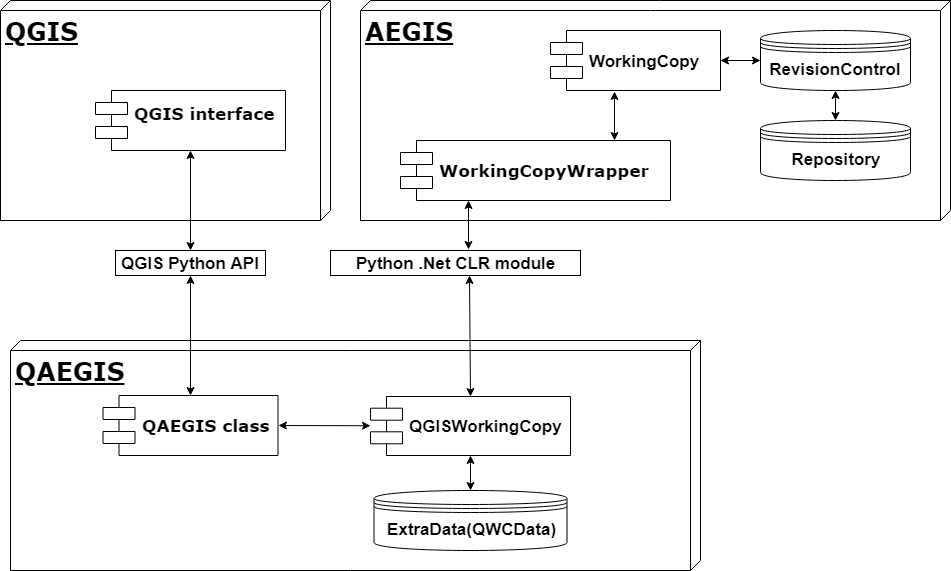
\includegraphics[width=0.8\textwidth,height=220px]{images/qaegis_component_diagram.png}
	\caption{A program komponensdiagramja}
	\label{fig:picture-7}
\end{figure}\todo{Betűméret növelés jól jönne erre az ábrára.}

\subsection{A geometriaadatok kezelése}
A geometriák tárolása, betöltése, valamint eltávolításuk kezelése mind az AEGIS létező funkciói voltak a projekt kezdeténél, így a tényleges feladat, a transzformációk definiálása, és létrehozása.
Az átalakítások tervezése közben az a fő szempont, hogy a lehető legáltalánosabbak legyenek, és minden lehetséges módosítás leírható legyen véges alkalmazásukkal. Ezt a törekvést segíti az, hogy az AEGIS geometriatípusai megfelelnek a \emph{Simple Feature Access} (röviden \emph{SFA}) standardnak \cite{sfa}, ezáltal egy adott hierarchiával rendelkeznek: a pontok különálló típust képeznek, a vonalláncok koordináták sorozatai, amik hasonlóan viselkednek a pontokhoz, a sokszögek pedig gyűrűkkel vannak leírva, amik a vonalak speciális változatai, így az "alacsonyabb szintű" geometriák transzformációi felhasználhatóak a bonyolultabb térobjektumok átalakításainak leírásához is. \todo{Fontos lenne hangsúlyozni, hogy az SFA modellben van egy geometria ősosztály / interfész, így egy teljes leszármazási hierarchia adott, minden geometriának van közös ős típusa.}
\begin{note}
A \emph{Simple Feature Access} geometriák tárolására és elérésére kialakított két részből álló szabvány. Az első rész (SFA-CA azaz \emph{Common Architecture}) egy modellt definiál a két dimenziós geometriáknak pontok közti lineáris interpolációval. Ez a rész definiálja WKT és WKB szabványos reprezentációkat is. A második rész a szabvány SQL alapú implementációját írja le. Az SFA standard az OGC (\emph{Open Geospatial Consortium}) és az ISO (\emph{International Organization for Standardization}) szervezetek által elfogadott.
\begin{figure}[H]
	\centering
	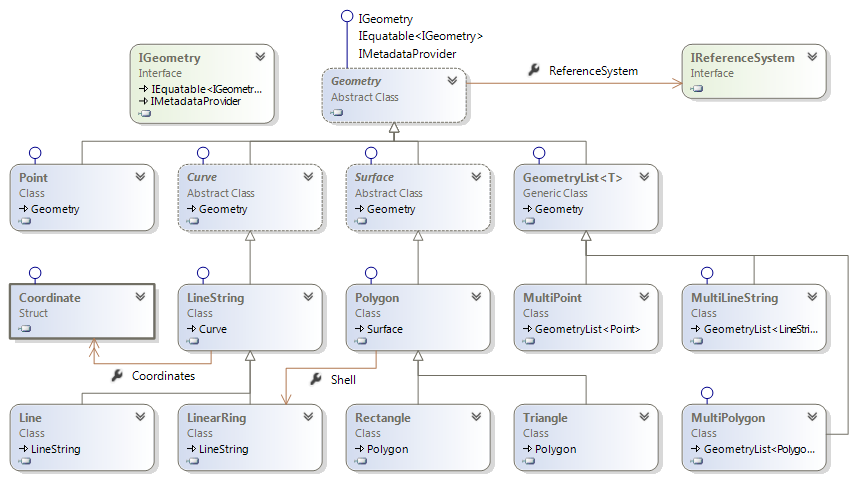
\includegraphics[width=0.8\textwidth,height=220px]{images/sfa.png}
	\caption{A \emph{Simple Feature Access} objektum-relációs modellje az AEGIS-ben}
	\label{fig:picture-8}
\end{figure}
\end{note}

 Az alakzatok lehetséges változásainak megfelelő rekreálásához a következő transzformációkat szükséges definiálni:
\begin{itemize}
	\item Pont eltolása
	\item Vonal részleges vagy teljes eltolása
	\item Pont felvétele a vonalba
	\item Pont eltávolítása a vonalból
	\item Sokszög héjának módosítása
	\item Sokszögben lévő lyuk módosítása
	\item Lyuk felvétele sokszögbe
	\item Lyuk eltávolítása sokszögből
\end{itemize}
Ezeken kívül az összes többi alakzatot egybefogó, úgynevezett multigeometriák változásainak leírásához szükségesek a következő műveletek:
\begin{itemize}
	\item Multigeometria egy vagy több részének módosítása a megfelelő egyedi geometria transzformációkkal
	\item Geometria hozzáadása multigeometriához
	\item Geometria eltávolítása multigeometriából
\end{itemize}
Ezen transzformációk segítségével bármilyen alapvető geometriaváltozást le lehet írni.

A transzformációk generálása komplex feladat, melynek során elemeznünk kell a kiindulási geometriát, és a végeredményt, ez alapján pedig létrehozni azt a transzformációgyűjteményt amit végrehajtva az eredetin, megkapjuk az újat. Vonalláncokra és poligonokra a következő algoritmussal adható meg:
\begin{enumerate}
	\item Tekintsük az eredeti és a módosult geometria komponenseinek számát (ld. \ref{sec:definitions}.~szakasz)
	\item A két geometria megegyező hosszú részein -- ami megegyezik a komponensszámuk minimumával -- hozzuk létre azokat a transzformációkat, amik az eredeti részeit az új részeknek megfelelő részekre alakítják
	\item Amennyiben az új geometria hosszabb, a régiben még nem létező részeket adjuk hozzá
	\item Amennyiben a régi geometria hosszabb, az újban már nem létező részeket töröljük ki
\end{enumerate}

Mivel pont geometriáknál csak az eltolás művelete létezik, nem szükséges részekre bontani a transzformációgenerálást, a koordináták különbségeiből kiszámolható az összes szükséges paraméter.

Ezen részek implementálásával a geometriák alakulásának követése megvalósítható.

\subsection{A QGIS reprezentáció kezelése}
A fő különbség az AEGIS és a QGIS geometriákat kezelő része között az, hogy az előbbi csak a téradatot kezeli, az utóbbi viszont ezeket még rétegekre osztva jeleníti meg. Ezzel önmagában nem lenne probléma, viszont a QGIS nem rendel egyedi azonosítót a geometriákhoz, így előfordulhat, hogy két különböző rétegen azonos geometria szerepel, és módosításukkor nem tudjuk megállapítani, hogy az AEGIS-ben tárolt adatok közül melyik módosult. Ez alapján  a beépülő modulon belül megvalósítandó plusz funkciók a következőek:
\begin{itemize}
	\item A QGIS objektumok (feature-ök) és az AEGIS geometriák kapcsolatának nyilvántartása
	\item A QGIS műveleteinek megfeleltetése az AEGIS műveleteknek
	\item Az AEGIS-ben tárolt állapotok megjelenítése 
	\item A verziókezelés lépéseihez grafikus kezelőfelület biztosítása
\end{itemize}

\section{Geometriai adatok változásának kezelése}
\subsection{Az AEGIS WorkingCopy}
Az AEGIS verziókezelő moduljának külső interfésze az úgynevezett \texttt{Working Copy}, avagy munkapéldány. Ezen kereszült a következő funkciók érhetőek el:
\begin{enumerate}
	\item Teljes revíziókezelő, és hozzá tartozó tároló létrehozása vagy betöltése, attól függően, hogy van-e már jelen egy
	\item Geometriák hozzáadása az aktuális verzióhoz
	\item Geometriák eltávolítása az aktuális verzióból
	\item Geometria módosítása az aktuális verzióban, az IGeometryTransformation interfészt megvalósító transzformációpéldánnyal
	\item Aktuális verzió mentése a verziókezelőbe
	\item Tetszőleges verzió betöltése és megjelenítése
\end{enumerate}
A WorkingCopy két hiányossággal rendelkezik a beépülő modulban való használathoz. Transzformációk előállítását nem támogatja, valamint az aktuális állapotát kifelé csak geometriák halmazaként biztosítja, ami a QGIS réteges megjelenítésében problémákat okozhat.
\subsection{Az AEGIS WorkingCopyWrapper}
A munkapéldány említett hiányosságainak pótlására jött létre a \texttt{WorkingCopyWrapper} osztály, amely a \texttt{WorkingCopy}-hoz képest az alábbi többletfunkciókkal bír:
\begin{enumerate}
	\item Eredeti és módosult geometria alapján transzformációk generálása, majd ezzel a workingcopy módosító függvényének használata
	\item Egy egyedi azonosítókkal ellátott geometrialista biztosítása a lokális állapotról
\end{enumerate}
A szükséges transzformációkat és generálásukat az AEGIS Processing könyvtárában kellett implementálni.
\subsection{A transzformációk}
A geometriák átalakító műveletek kialakítása az alábbi elven alapul:
\begin{itemize}
	\item A pontok transzformációja leírható egy egyszerű vektor hozzáadással
	\item Az összes többi geometria kisebb részekből áll (ld. \ref{sec:definitions}.~szakasz)
	\item Egy geometria módosítása leírható a részeire vonatkozó kisebb transzformációkkal
\end{itemize}
Ez alapján három típusú transzformáció alakult ki: $i)$ a rész módosítása, ami a módosítandó részek indexeit és a részeken elvégzendő résztranszformációit tartalmazza; $ii)$ a rész hozzáadása amely az új rész geometriáját és a beszúrás indexét tartalmazza; $iii)$ valamint a rész eltávolítása, amely az eltávolítandó rész indexét tárolja, valamint az eltávolított rész geometriáját, erre az invertálhatóság megvalósításához van szükség.
\subsection{Az IGeometryTransformation interfész}
Ahogy korábban is említésre került, az AEGIS a transzformációkat az IGeometryTransformation \todo{Több helyen a típusnevek / metódusok nincsenek megfelelő betűtípussal szedve, ezeket ellenőrizd.} implementációjaként várja. 
\begin{figure}[H]
	\centering
	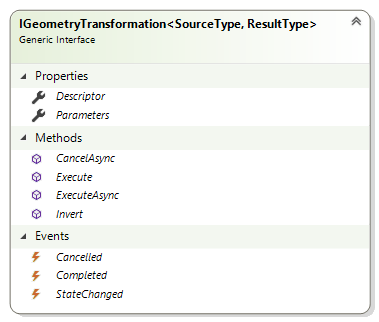
\includegraphics[width=\textwidth,height=250px]{images/GeomTransformIface.png}
	\caption{A geometriatranszformációs interfész osztálydiagramja}
	\label{fig:picture-9}
\end{figure}\todo[inline]{Ezt nem lehetne VS-sel generálni? Egységes lenne az osztálydiagramok stílusa akkor. Ha nem lehet, akkor csak legyen kicsit kisebb, mert túl nagy a betűméret.}

Ezen interfész legfontosabb metódusai:
\begin{enumerate}
	\item \texttt{Execute(IGeometry geometry)}: a transzformáció végrehajtása az \texttt{IGeometry} interfésznek megfelelő téradaton, a módosított alakzat visszaadása. A forrásgeometriának meg kell egyeznie a transzformáció bemeneti típusával.
	\item \texttt{Invert()}: A transzformáció inverzének előállítása, mellyel helyreállítható az eredeti geometria. Hozzáadás típusú művelet inverze ugyanazon az indexen történő eltávolítás és fordítva, részmódosítás esetén a résztranszformációk inverzeinek végrehajtása ugyanazokon a részeken.
\end{enumerate}
Az összes módosítást leíró osztály rendelkezik ezen metódusok egyedi implementációival, melyek megfelelnek a saját geometriatípusaiknak.
\subsection{A transzformációk generálása}
Az eredeti és módosított geometriákból transzformációk generálását az AEGIS Processing modulban található TransformationFactory statikus osztályok végzik.
A transzformációk létrehozása a specifikációban leírt algoritmus alapján működik, ez az alábbi pseudokóddal szemléltethető:
\begingroup
\lstset{
	caption={A transzformációgenerátorok általános algoritmusa},
	label=src:transformgeneric,
	numbers=none,
	backgroundcolor=\color{white},
	frame=single
}
\begin{lstlisting}
set unmodifiedCount to number of parts in unmodified geometry
set modifiedCount to number of parts in modified geometry
set result to new empty transformation list
for index := 0 to minimum(unmodifiedCount, modifiedCount) do
	create transformation from parts on the index and add to result
for index := unmodifiedCount to modifiedCount do
	create addition for new parts and add to result
for index := modifiedCount to unmodifiedCount do
	create deletion for removed parts and add to result
return the result
\end{lstlisting}
\endgroup
\todo[inline]{Ezt a pseudokódot inkább úgy lett volna jó formázni, ahogyan a minta doksi 13. oldalán van az algoritmus:\\
\url{https://github.com/mcserep/elteikthesis/blob/master/thesis.pdf}\\
Kicsit javítottam a formázásán, ha ez maradna, de kicsit olyan, mintha angol szöveget írtál volna a magyar dolgozatba.}
Mint látható, a generáló függvény először létrehoz annyi résztranszformációt, amekkora részen még egyezik a két geometria hossza, majd a még nem, vagy már nem jelen lévő részgeometriák létrehozásának illetve eltávolításának műveleteit állítja elő. Az összes transzformációgenerátor hasonló módon működik.

\section{C\# folyamatok használata Python kódban}
Ahogy a specifikáció elején említésre került, a szoftver amihez a verziókezelő beépülő modul és a verziókezelést biztosító könyvtár két teljesen különböző technológiát használ. Mivel a Python programozási nyelv széleskörűen elterjedt különböző extra funkciók hozzáadására más környezetekhez, ezért több opció volt az eltérő megoldások összekötésére. Az egyik az IronPython nevű kiegészítő modul a Pythonhoz, viszon ez csak a nyelv 2.7-es verzióját támogatja, aminek hamarosan megszűnik a támogatottsága, így más utat kellett keresni. Az előbbihez hasonlóan nyílt forráskódú Python.NET modul azonos funkcionalitással rendelkezik, és a legújabb verziókkal is kompatibilis, így kézenfekvő megoldásnak bizonyult. A Python.NET projekt integrálása a QGIS pluginba egyedül azért okozott nehézséget, mivel a nyelvi összeköttetést biztosító szoftver fordításához számos dependenciának jelen kell lennie a rendszerben, így végül már fordított bináris formájában került a beépülő modulba. Ez sajnos kizárja annak lehetőségét, hogy a könyvtár esetleges frissülésével a plugin is dinamikusan megkapja a legújabb állományokat, viszont a program telepítését meglehetősen megkönnyíti.
\subsection{A Python.NET használata}
A Python.NET az úgynevezett \emph{Common Language Runtime} (\emph{CLR}) modult biztosítja a Python programozási nyelvhez. Amennyiben a fordított források a Python belső elérési útvonalain szerepelnek, importálható a CLR modul. Ezután a szintén classpathhoz adott dinamikusan linkelhető szoftverkönyvtárba (DLL) fordított C\# könyvtárakat is hozzáadhatjuk a Python kódhoz. A tényleges implementációban a beágyazás az alábbi módon néz ki :
\lstset{caption={A CLR modul bekötése, és a DLL fájlok importálása a Q-Aegis kódjában}, label=src:pythonload}
\begin{lstlisting}[language={python}]
pluginpath = "{}/../python/plugins/qaegis".format(QgsApplication.pluginPath())
sys.path.insert(0,pluginpath+"/pythonnet")
sys.path.insert(0,pluginpath+"/aegis")

import clr
clr.AddReference('AEGIS.Core')
clr.AddReference('AEGIS.IO')
clr.AddReference('AEGIS.Versioning')
clr.AddReference('AEGIS.Processing')
\end{lstlisting}
Az importálás után pedig például ilyen módon hozhatunk létre egy String kulcsokkal egész számokat tároló C\# szótárat:
\lstset{caption={C\# objektum használata Python kódban}, label=src:pythoninstantiate}
\begin{lstlisting}[language={python}]
dictionary =  Dictionary[String,int]()
\end{lstlisting}

\section{Adatátvitel Python és C\# közt}
A geometriák ugyan az AEGIS és a QGIS rendszerekben is szabványosan vannak kezelve, viszont a megvalósításaik különbözőek. Az ebből adódó problémák elkerülése érdekében a geometriák a legtöbb helyen a WKT reprezentációjukban, szövegesen kerülnek átadásra. Ezen kívül az AEGISben a geometriákhoz rendelt egyedi azonosító is használva van néhány helyen az objektumok kiválasztására. Erre azért van szükség, mert az AEGIS a geometriák közti ellenőrzésekor sokkal pontosabb adatokkal dolgozik mint a QGIS és ezek az eltérések sokszor nem várt viselkedéseket eredményeztek, például geometriák módosításakor a verziókezelő modul ellenőrzi, hogy van-e a módosított geometriával egyező a tárolóban, és ha nem talál ilyet, akkor szimplán felveszi újként, ami a pontatlanságok miatt lehetetlenné tette a módosítások hatékony követését, ezért módosításkor az eredeti állapotot közvetlenül kulcs alapján szedi ki a rendszer a tárolóból, ahelyett hogy a QGIS reprezentációval egyező geometriát keresne.

\section{A QgisWorkingCopy}
\subsection{A  hiányzó információk biztosítása}
Az AEGISben létrehozott kibővített munkapéldány önmagában még nem elég ahhoz hogy a QGIS projektek verziókezelésére alkalmas legyen, mivel nem képes a rétegek adatainak és változásainak követésére, valamint nincsen megoldása arra se, hogy a különböző featureökhöz rendelje a benne tárolt geometriákat. Ezeket a funkciókat a QgisWorkingCopy Python osztály biztosítja az úgynevezett QWCData állomány segítségével. Ebben egy extraData névre keresztelt objektum található amely az alábbi formátumot követi:
Az egész objektum egy Python szótár, amelyben a kulcsok a verziószámok, a hozzájuk tartozó objektumok pedig a projekt adott verzióhoz tartozó állapotát írják le. Ebben az állapotleíróban a keyDict a featureök Qgis azonosítójához (ld. \ref{sec:definitions}.~szakasz) rendelve tárolja az Aegisben tárolt geometriák kulcsait, a layers pedig a rétegek betöltéséhez szükséges adatokat tartalmazza: az azonosítót, a geometriatípust és a referenciarendszert.
\subsection{A QGIS munkapéldány funkciói}
\subsubsection{Extra adatok nyilvántartása}
a QgisWorkingCopy tükrözi az AEGIS munkapéldány wrapper funkcionalitását, kiegészítve azokat az extra adatok karbantartásával. Példányosításakor ellenőrzi, hogy létezik-e a verziókezelő állományainak tárolására mappa, ha nem létrehozza, majd példányosítja a wrappert, szimpla fájl alapú tárolóval és kétirányú deltákat használó revízió kontrollerrel. Ezek után betölti az azonos mappában tárolt QWCData fájlból a szükséges további adatokat.
A geometriák hozzáadása, módosítása és törlése egyszerűen a WorkingCopyWrapper azonos metódusait hívja meg, azonban a commit függvény hívásakor el kell tárolnia az extra adatokat. Ezen információk a Q-Aegis futása közben gyűlnek össze mely folyamat később lesz részletezve. A legtöbb adat kezelése nyílvánvaló, viszont a feature azonosítók karbantartása, valamint a verziók betöltése érdemel némi külön figyelmet.
\subsubsection{A feature azonosító probléma}
A QGIS a rétegeken lévő objektumok azonosítóit a réteg tárolásától függően különböző módon kezeli (amire a dokumentációja nem sok említést tesz). Amennyiben memóriában tárolt a réteg , a \emph{feature}-ök indexelése 1-től kezdődik, és a műveletektől függetlenül nem változik. \emph{Shapefileban} tárolt adatok esetén viszont 0-tól indul az indexelés, és objektum eltávolítása esetén az összes olyan azonosító, ami nagyobb volt nála, csökken eggyel, hogy egy folyamatos azonosító állapot maradjon. Ezért amikor \emph{feature} eltávolításokat kezelünk, és a réteg tárolója shapefile volt, minden törlés után az összes eltárolt nagyobb azonosítót dekrementálni kell eggyel.
\subsubsection{Verzió betöltése, rétegek kezelése}
Egy kiválasztott verzió betöltése a munkapéldányon keresztül történik, először a \emph{workingcopy}-t a megjeleníteni kívánt verzióra állítjuk, majd ebből lekérjük az aktuális geometria állapotot, amit a geometriák egyedi azonosítóiból és magukból a geometriákból álló párok formájában kapunk meg, C\# szótár formájában. Ezt az adott verzióhoz tartozó extra adat objektum segítségével feldolgozzuk olyan módon, hogy rendelkezésünkre álljon az összes megjeleníteni kívánt réteg létrehozásához szükséges adat, valamint összepárosítjuk a \texttt{keyDict} segítségével a geometriákat a layereken kirajzolandó featureökkel. Ezt követően a rétegadatok alapján létrehozzuk a valódi QGIS rétegeket, feltöltjük őket az adott verzióban lévő állapotukkal, majd ezeket jelenítjük meg a QGIS grafikus felületén.

\section{A QAEGIS osztály}
A tényleges beépülő modul maga a QAEGIS Python osztály, melynek váza a QGIS-hez írt plugin builder beépülővel lett generálva. Ez biztosítja, hogy az alap szerkezete megfelelő legyen az alapprogramba való integráláshoz, és minden szükséges metaadattal rendelkezzen. Ebben az osztályban férünk hozzá a QGIS interfészéhez, amin belül az aktuális projekt példánnyal dolgozik a modul. Mivel a QGIS grafikus felülete a Qt szoftverkönyvtáron alapul, ezért az események kezelésére az úgynevezett \emph{szignálokat} használjuk fel. A szignálokat a felhasználó tevékenységei váltják ki, és egy adott információhalmazt adnak, amire ráköthetünk saját implementálású feldolgozófüggvényeket. A szignálok és kezelésük áttekintésével könnyen megérthető a beépülő modul működése.
\subsection{Szignálok és feldolgozásuk}
\subsubsection{A QGIS interfész projekt megnyitási szignál}
Ezen jelzést használja a modul a munkapéldány megnyitására, amely folyamat vagy létrehoz egy új üres revíziókezelőt, vagy ha létezik a megnyitott projekthez egy, betölti azt. Ezen szignál kezelése során jönnek létre azok a listák is amik követik az aktuális szerkestésekben a rétegek és featureök létrehozását és törlését.
\subsubsection{A projekt példány réteg szignáljai}
Az aktuálisan megnyitott projekt réteg létrehozásakor vagy törlésekor egy jelzés formájában ad információkat a végzett műveletről. Ezeket kezelve kerülnek a bufferlistákba az elvégzett műveletek. A bufferekre azért van szükség, mert a projekt mentéséig nem tekinthető véglegesnek a réteg jelenléte vagy eltávolítása, ezért amíg nem mentett állapotban vannak, nem kerülnek be a revíziókezelésbe. A réteg törléséhez tartozó szignál kezelésekor nem csak a rétegadatok eltávolítása kerül a bufferbe, hanem az összes rajta lévő objektum törlése is, így ha a layer már nincs jelen, a tartalma se marad felesleges adatként a rendszerben.
\subsubsection{A projekt mentésének szignálja}
A projekt mentésekor tekinthető ténylegesen elvégzettnek egy layer törlése vagy felvétele, ezért ezen jelzés kiváltásakor kerülnek ezek a módosítások a munkapéldányba. Új rétegek esetén a rajtuk végzett geometriaműveletek mentésig nem relevánsak -- hiszen ha elvetnénk a mentésüket, az összes rajtuk lévő objektum is törlésre kerülne --, így mentés után kerül be minden feature is új geometriaként az AEGIS rendszerbe.
\subsubsection{Réteg mentésekor kiváltott jelzések}
Fontos megjegyezni, hogy a rétegek rendelkeznek az egyes műveletek végrehajtásakor megjelenő szignálokkal is, viszont ezek nem biztos hogy mentésre is kerülnek, így hasonlóan a rétegműveletek buffereléséhez, ezek is egy köztes állapotban tárolódnak a véglegesítésükig. Szerencsére ezt a funkciót maga a QGIS biztosítja, így a függőben lévő műveletek tárolását nem szükséges újraimplementálni.A rétegen végzett műveletek mentésekor három különböző jelzés kerül feldolgozásra.
\begin{list}{}{}
	\item $\bullet$ \textbf{Hozzáadott featureök mentése}: Ezen szignál szolgáltatja az adatokat az újonnan létrehozott geometriákról, így ezen keresztül kerülnek be az új téradatok a verziókezelésbe. Érdemes kiemelni itt az alábbi kódrészletet : 
	\lstset{caption={A multigeometria réteg probléma kezelése}, label=src:python}
	\begin{lstlisting}[language={python}]
	geomToAdd = feature.geometry()
	for layer in self.iface.mapCanvas().layers():
		if layer.id() == layerId:
			layerType = layer.wkbType()
	if layerType in range(4,7) :
		geomToAdd.convertToMultiType()
	\end{lstlisting}
	Erre azért van szükség, mert amennyiben a réteg multigeometriákkal dolgozik, új geometria létrehozásakor -- valamilyen ismeretlen okból -- még szimpla téradatként kezeli azokat, viszont bármilyen módosítást végzünk rajtuk, átalakítja az egyszerű alakzatokat egyelemű többszörös változataikká. Ez komoly problémákat tud okozni a módosítások kezelésénél, hiszen követetlenül változik meg a geometria típusa. Ezért ellenőrzi a program, hogy a réteg geometriatípusa többszörös-e, amit a 4,5,6 kódokkal jelöl, és ha igen, akkor még az új adat bekerülése előtt konvertálja azt multigeometria formába.
	\item $\bullet$ \textbf{Eltávolított featureök mentése}: A geometriák eltávolításakor problémás, hogy az újonnan létrehozott adatokat mentésükig ideiglenes azonosítóval kezeli a QGIS, és mentéskor ezeket az ideiglenes változatokat törli, és felveszi véglekesként. Mivel az ideiglenes verzióik nem szerepelnek a verziókövetésben, így ha az eltávolításukat próbálnánk feldolgozni, hibára futnánk. Ezt kiküszöbölendő kihasználjuk az ideiglenes featureök egy tulajdonságát. Amíg a már véglegesített objektumok tárolás módjától függően 0-tól vagy 1-től kezdve kapnak azonosítót, ideiglenes verzióik a negatív irányba kapnak azonosítót (ID-t), ezért ha egy feature azonosítója 0 vagy 1 alatti, ideiglenesnek tekinthető. Ennek felhasználásával megfelelő módon eltávolíthatóak a ténylegesen a felhasználó által törölt téradatok.
	\item $\bullet$ \textbf{Módosítótt geometriák mentése}: A módosított geometriák kezelése elég egyértelmű mivel a valódi változáskezelést az AEGIS kiegészítései biztosítják, az egyedüli plusz ellenőrzés ami belekerült azt vizsgálja, hogy a módosított geometria mentetlen rétegen foglal-e helyet, és ha igen, nem tekintjük módosításnak, hiszen még nem került be a rendszerbe.
\subsubsection{A projekt bezárásának szignálja}
A projekt bezárásakor fontos, hogy az összes jelzésről leiratkozzon a program, ugyanis ennek hiányában a QGIS implementációjából kifolyólag egy másik projekt megnyitásakor a különböző szignálok többszörösen kerülnének kezelésre, ami nem kívánt működéshez vezet.
\end{list}
\subsection{A kezelőfelület és eseményei}
A kezelőfelület alapja a plugin generátor által létrehozott Qt ablak, amely Qt designer segítségével lett végleges formájára alakítva. A felület tervezésekor a fő szempont az volt hogy annyira egyszerű és intuitív legyen amennyire az csak lehetséges, így végül mindössze két elemmel vezérelhetővé vált a teljes verziókezelés
\begin{enumerate}
	\item \textbf{A commit gomb}: Az aktuális verzió mentésére szolgáló gomb kettős funkciót tölt be. Az általánosabb, hogy ha már kezelt projekttel dolgozuk, megnyomásakor változtatásaink véglegesítésre kerülnek a revíziókezelő modulban, és létrejön egy újabb verzió. Másik funckióját abban az esetben látja el, ha egy létező, de még nem verziókezelt projekt van megnyitva. Ekkor megnyomásával a projekt teljes szerkezete, azaz rétegei és azok tartalma bekerülnek a friss munkapéldányba mint kiindulási verzió.
	\item \textbf{A verzióválasztó lista vagy beviteli mező, és a hozzá tartozó betöltés gomb}: A verzióválasztó vezérlőelem nem jelenik meg a kezelőfelületen addig, amíg a munkapéldány nem rendelkezikbetölthető verzióval. Amennyiben már használható, a kívánt verziószámot kiválasztva és a betöltőgombra kattintva elindul a kiválasztott revízió megjelenítése. Mivel a verziómegjelenítés implementációjából fakadóan elveti az összes aktuális módosítást amit esetlegesen még nem mentett a felhasználó, ezért amennyiben vannak ilyen függőben lévő műveletek, a program felajánlja azok mentését egy új verzióba a betöltés megkezdése előtt.
	\begin{note}
	A verzióválasztó elem attól függően, hogy mennyi verzió érhető el, két alakot vehet fel : kevesebb verzió esetén egy legördülő menü, bizonyos darabszám fölött pedig egy léptethető szám beviteli mező. Lista esetén egyértelműen nem választható ki hibás adat, léptetőmező esetén pedig megfelelő minimum és maximum értékek megkötésével biztosított, hogy nem ad meg a felhasználó nem létező verziószámot.
	\end{note}
\end{enumerate}

\section{A program fájlszerkezete}
\subsection{A nyers programkód}
A létrehozott programkód szerkezete szétválasztható a C\#-ban valamint a Pythonban írt részekre.\\
A C\# nyelven implementált kód az alábbi struktúrát követi:
\begin{enumerate}
	\item Az AEGIS egyes funckinalitásai a megfelelő könyvtárakban található állományokban vannak
	\item A geometriatranszformációk, valamint a transzformációgenerátorok osztályai az AEGIS Processing könyvtárának \texttt{QgisTransformation} alkönyvtárában kerültek mentésre
	\item A munkapéldány wrapper osztálya az AEGIS Versioning \texttt{WorkingCopy} könyvtárában lett létrehozva, az általa használt eredeti \texttt{WorkingCopy} mellett 
\end{enumerate}
A Python kód a qaegis mappában található, az alábbi szerkezetel:
\begin{enumerate}
	\item A plugin magját adó \texttt{QAEGIS} osztály definícióját, valamint a \texttt{QgisWorkingCopy} osztályt a qaegis.py állomány tartalmazza
	\item A szükséges konverziók implementációi a converters.py fájlban találhatóak
	\item A kezelőfelület leírása a \texttt{qaegis\_dialog.ui} állományba, a működtetéséhez szükséges kód az azonos nevű de Python kiterjesztésű fájlba került
\end{enumerate}
\subsection{A működéshez szükséges binárisok}
A beépülő modul működéséhez szükséges az AEGIS csomag dllekké fordított verziója a plugin könyvtáron belüli aegis mappában kapott helyet, a lefordított Python.NET CLR modul pedig az azonos szülőmappájú \texttt{pythonnet} könyvtárban található.

\section{A működésben lévő beépülő modul könyvtárszerkezete}
A használatban lévő plugin a QGIS Python beépülőket tartalmazó mappájában található, ebben a könyvtárban van minden szükséges állomány. A tényleges verziókezelést biztosító tárolók a kezelt projektet tartalmazó mappában kerülnek létrehozásra, egy \texttt{projektnév\_qaegis\_repository} nevű mappában, ezen belül pedig a kezelt projekt nevével megegyező mappákban találhatóak a szükséges fájlok. Ezen belül a changesets mappa verziószámokkal elnevezett forrásaiban találhatóak a revíziókhoz tartozó változáslisták, a snapshots mappa tartalmazza az esetlegesen mentett verzióállapotokat, a revisioncontrol fájl pedig az összes többi használt adatnak ad helyet. A QWCData állomány tartalma az összes AEGIS-en kívüli követendő adat szerializált formája.

\section{A program fordítása}
A program fordítása három lépésből áll: Az AEGIS fordítása, a Python.NET fordítása, végül pedig a plugin deploy.
\subsection{Az AEGIS modulok fordítása}
Az AEGIS-ben található források fordítása értelemszerű C\# fordítás. A fordítás után keletkezett dll állományokat át kell másolni a plugin munkakönyvtárának aegis almappájába
\subsection{A Python.NET fordítási környezet előkészítése}
A QGIS architektúrája miatt -- ami saját belső verziót használ a Python nyelvből -- a \emph{Python.NET} CLR\todo{A CLR egy rövidítés, nagybetűkkel kell írni.} modul fordításához több előzetes lépést is végre kell hajtani:
\begin{enumerate}
	\item A QGIS-t az OSGeo4W telepítőn keresztül kell installálni, a setuptools, pyrcc5 csomagokkal együtt
	\item Az OSGeo4W shellt megnyitva futtatni kell a bin könyvtárban található \emph{py3\_env.bat} valamint \emph{qt5\_env.bat} fájlokat
	\item ezután a setuptools által biztosított easy\_install parancs segítségével telepítsük a pip-et
	\item a pip segítségével telepítsük a wheel modult.
\end{enumerate}
Ezek után lépjünk be a pythonnet könyvtárba, és fordítsuk le a következő paranccsal: \verb|python setup.py build\_ext --inplace|
\begin{note}
A Python.NET\todo{Legyen következetes az elnevezés: Python.NET. Ne Python .Net és ne pythonnet.} fordításához a felsorolt lépéseken kívül szükséges még a .Net keretrendszer 3.5-ös verziója, ami már nem alapértelmezetten része a Windows operációs rendszernek, valamint szükséges a Windows SDK vagy egy Visual Studio jelenléte is a számítógépen. Mindezeken felül a pythonnet fordítása során használt \emph{UnmanagedExports} modul miatt a rendszer nyelve angol kell hogy legyen, ez azt jelentheti, hogy az operációs rendszert újra kell telepíteni angol nyelven.
\end{note}
\subsection{A plugin fordítása (\emph{deploy})}
Ha lefordítottuk az AEGIS és Python.NET modulokat, akkor a \texttt{pb\_tool deploy} paranccsal fordíthatjuk le a Python kódból valamint ui fájlokból származó forrásokat. Ez a parancs be is másolja a QGIS plugin könyvtárába a beépülő modult.

\section{Tesztelés}
A tesztelés hagyományos feketedoboz típusú tesztelésként történt, az alábbi tesztelési terv mentén:
\begin{center}
	\begin{longtable}{ | p{0.5\textwidth} | p{0.5\textwidth} | }
		
		\hline
		\emph{Végrehajtott művelet} & \emph{Várt viselkedés}
		\\ \hline \hline
		\endfirsthead % első oldal fejléce
		
		\hline
		\emph{Végrehajtott művelet} & \emph{Várt viselkedés}
		\\ \hline \hline
		\endhead % többi oldal fejléce
		
		
		\emph{Megnyitott projekt nélkül a verziókezelő ablak megnyitása}
		& Az ablak nem nyílik meg, a felhasználó kap egy üzenetet, hogy projekten kívül nem használhatóak a verziókezelési funkciók
		\\ \hline
		
		\emph{Új projekt létrehozása mentés nélkül}
		& Hibaüzenet jelenik meg, ami jelzi a felhasználónak, hogy projektfájl nélkül nem használható a verziókezelés
		\\ \hline
		
		\emph{Új projekt létrehozása mentéssel}
		& A projekt mentésre kerül, elérhető a verziókezelő ablak, a verzióválasztó és a betöltőgomb nélkül
		\\ \hline
		
		\emph{A commit gomb megnyomása a legutóbbi verzión álló verziókezeléssel}
		& Az előző verzió óta végrehajtott változtatások mentésre kerülnek, bezárul a verziókezelő ablak, a felhasználó kap egy üzenetet, hogy a mentés sikeres.
		\\ \hline
		
		\emph{A commit gomb megnyomása régebbi verzión álló verziókezeléssel}
		& A változtatások mentése nem történik meg, a felhasználót hibaüzenet értesíti arról, hogy csak a legutóbbi verzión menthetőek módosítások.
		\\ \hline
		
		\emph{Nem verziókezelt projekt megnyitása, majd a commit gomb megnyomása}
		& A projekt megnyitásakor létrejön egy üres tároló, a commit gomb megnyomása után az összes réteg és tartalmuk bekerül a verziókezelésbe
		\\ \hline
		
		\emph{Verziókezelt projekt megnyitása}
		& A projekt betöltése után a verziókezelő a legutóbbi állapotra áll, elérhető a korábbi verziók betöltése, valamint a módosítások mentése.
		\\ \hline
		
		\emph{Korábbi verzió betöltése, mentetlen módosítások nélkül}
		& A régebbi állapotnak megfelelően létrejönnek a rétegek és a rajtuk lévő geometriák, a verziókezelő ablak bezárul.
		\\ \hline
		
		\emph{Korábbi verzió betöltése, mentetlen módosításokkal}
		& A program megnyit egy párbeszédablakot, amelyben figyelmezteti a felhasználót, hogy a verzió betöltésével a még nem commitolt módosításai elvesznek, és felajánlja ezek mentését. Ezután a verzió betöltése megtörténik.
		\\ \hline
		
		\emph{Bármilyen aktuális verziószám változásával járó művelet}
		& Az aktuális verziót feltűntető mező a megváltozottra frissül
		\\ \hline
		
		\emph{Réteg hozzáadása a projekthez, majd a változtatások mentése}
		& A réteg hozzáadása mentésre kerül, a létrehozás verziójától kezdve betöltésnél megjelenik
		\\ \hline
		
		\emph{Réteg eltávolítása a projektből, majd a változtatások mentése}
		& A réteg törlése mentésre kerül, a törlés verziójától kezdve betöltésnél nem jelenik meg
		\\ \hline
		
		\emph{Geometriák módosítása, a réteg mentése, majd a változtatások commitolása}
		& A geometriák módosítása mentésre kerül, minden verzióban az adott verziónak megfelelő állapotban kerülnek betöltésre
		\\ \hline
		
		\emph{Geometriák módosítása, a réteg mentése nélkül, majd a változtatások commitolása}
		& A módosítások nem kerülnek mentésre (mivel nem véglegesek)
		\\ \hline
		
		
		
		\caption{A tesztelési terv}
		\label{tab:example-3}		
	\end{longtable}
\end{center}

\section{Továbbfejlesztési lehetőségek}
\subsection{Az AEGIS továbbfejlesztési lehetőségei}
Az AEGIS szerkezetéből adódóan számos lehetőséget biztosít további funkciók létrehozására:
\begin{enumerate}
	\item A geometriákhoz tartozó egyéb metaadatok módosítására létre lehetne még hozni új transzformációs osztályokat, ezáltal ezek is kezelhetőek lennének
	\item A módosítások kezelését tovább lehetne fejleszteni olyan adatok hozzáadásával, mint a szerkesző felhasználó azonosítója, ezzel alkalmasabbá téve a verziózást több ember által végzett projektek esetén is.
	\item Esetlegesen a rétegrendszer implementálható lenne az AEGIS-en belül, mivel a legtöbb vektorgrafikus szoftver hasonló elven működik, így nem az alkalmazás részben kéne ezeket az információkat kezelni.
\end{enumerate}
\subsection{A Python modul továbbfejlesztése}
\begin{enumerate}
	\item A QAEGIS és QgisWorkingCopy osztályok erőteljesen az AEGIS keretrendszerre támaszkodnak, ezért annak bármilyen kiegészítése implementálható lenne ezen beépülő modulban való alkalmazásra is.
	\item A kezelőfelület bővíthető lenne egy, a verziókezelők exportálására és importálására alkalmas funkcióval, így nem kéne az állományok másolását alkalmazni projekt betöltésére.
	\item Mivel a QGIS a geometriák megjelenítésének vizuális részleteit, például a színüket, a rétegekhez kötve szabályozza, a rétegek stílusának követésével pontosabb állapotbetöltésre lenne lehetőség
\end{enumerate}

\section{Fogalomtár}
\label{sec:definitions}

\begin{description}
	\item[Feature]: A QGIS geometriai egysége, a rétegen tárolt geometria és az összes hozzá tartozó egyéb adat.

	\item[Geometriatípus]: A szabványos geometrialeírás típusainak egyike, lehetséges értékei Point, MultiPoint, LineString, MultiLineString,Polygon,MultiPolygon \todo{Típusok formázása hiányzik.}.

	\item[Geometria komponenseinek száma]: A geometria közvetlen részgeometriáinak száma. Vonal esetén a pontjainak száma, sokszög esetén 1 (azaz a héj számossága) + a hozzáadott lyukak száma stb.

	\item[Geometria részgeometriái]: Pont geometriának nincs részgeometriája. Vonal geometria részei a pontok amelyek összekötésével megkapjuk a vonalat. Sokszög esetén az alakzat külső héja, valamint a síkidomon lévő lyukak, ezek vonalakkal írhatóak le. Multigeometriák részgeometriái az egyes különálló részeik.

	\item[Layer]: A QGIS megjelenítési rétege, kötött geometriatípussal, projekten belül tetszőleges darabszámú létezhet.

	\item[MultiGeometria]: Olyan geometria, amely több különálló geometriát tartalmaz, de egy egységként van kezelve.

	\item[Project]: A QGIS munkapéldánya, rétegeket lehet hozzáadni, és azon geometriákkal lehet műveleteket végezni.

	\item[WKB,WKT]: \emph{Well Known Binary}, \emph{Well Known Text}, geometriák leírására használt szabványos bináris és szövegformátum \cite{sfa}.

	\item[Working Copy]: A munkapéldány a verziókezelésen belül, egy adott verzió állapotát tartalmazza, a legfrissebb verzión szerkeszthető.

	\item[Qgis azonosító]: A featureök egyedi beazonosítására használt karakterlánc, a réteg azonosítójából és a feature azonosítójából áll elő.

	\item[Szótár adatszerkezet]: Kulcs-érték párokat tartalmazó lista. C\#-ban kötött a kulcsok és értékek típusa, Pythonban akár elemenként eltérhet.
\end{description}
\cleardoublepage

\chapter{Összegzés}
\label{ch:sum}

Lorem ipsum dolor sit amet, consectetur adipiscing elit. In eu egestas mauris. Quisque nisl elit, varius in erat eu, dictum commodo lorem. Sed commodo libero et sem laoreet consectetur. Fusce ligula arcu, vestibulum et sodales vel, venenatis at velit. Aliquam erat volutpat. Proin condimentum accumsan velit id hendrerit. Cras egestas arcu quis felis placerat, ut sodales velit malesuada. Maecenas et turpis eu turpis placerat euismod. Maecenas a urna viverra, scelerisque nibh ut, malesuada ex.

Aliquam suscipit dignissim tempor. Praesent tortor libero, feugiat et tellus porttitor, malesuada eleifend felis. Orci varius natoque penatibus et magnis dis parturient montes, nascetur ridiculus mus. Nullam eleifend imperdiet lorem, sit amet imperdiet metus pellentesque vitae. Donec nec ligula urna. Aliquam bibendum tempor diam, sed lacinia eros dapibus id. Donec sed vehicula turpis. Aliquam hendrerit sed nulla vitae convallis. Etiam libero quam, pharetra ac est nec, sodales placerat augue. Praesent eu consequat purus.

\cleardoublepage

% Irodalomjegyzék - kötelező
\addcontentsline{toc}{chapter}{\biblabel}
\printbibliography[title=\biblabel]
\cleardoublepage

% Ábrajegyzék - ha szükséges
\addcontentsline{toc}{chapter}{\lstfigurelabel}
\listoffigures
\cleardoublepage

% Táblázatjegyzék - ha szükséges
%\addcontentsline{toc}{chapter}{\lsttablelabel}
%\listoftables
%\cleardoublepage

% Forráskódjegyzék - ha szükséges
\addcontentsline{toc}{chapter}{\lstcodelabel}
\lstlistoflistings

\end{document}
